\def\year{2015}
%File: formatting-instruction.tex
\documentclass[letterpaper]{article}
\usepackage{graphicx}
\usepackage{algorithm}
\usepackage{algpseudocode}
\usepackage{pifont}
\usepackage{amsmath}
\usepackage{aaai}
\usepackage{times}
\usepackage{helvet}
\usepackage{courier}
\usepackage{float}
\frenchspacing
\setlength{\pdfpagewidth}{8.5in}
\setlength{\pdfpageheight}{11in}
\pdfinfo{
/Title (Group Anomaly Detection using Hierarchal Model)
/Author (Put All Your Authors Here, Separated by Commas)}
\setcounter{secnumdepth}{1}  
 \begin{document}
% The file aaai.sty is the style file for AAAI Press 
% proceedings, working notes, and technical reports.
%
\title{Hierarchical Bayesian Network for Group Anomaly Detection}
\author{Tadesse Zemicheal and Amran Siddiqui\\
{zemichet,siddiqmd}@eecs.oregonstate.edu\\
Oregon State University, Corvallis OR\\
}
\maketitle
\begin{abstract}
\begin{quote}
In most problem of anomaly detection, the main interest is, finding point anomalies. But, in some domain unusual pattern in data can only be detected when the distribution of a group of points are considered as a whole. \\
In this project, we tried a generative hierarchical Bayesian model for detecting group anomalies. We tried the proposed model and extend to find group type for groups on synthetic data and real dataset from ADAMS data and Weather data. The proposed model performs well in synthetic data, but the result from real dataset was not satisfactory.  
\end{quote}
\end{abstract}

\section{Introduction}
Anomalies are data points those don't conform to the majority pattern of the data. In most Anomaly detection problem, the goal is to identify these points anomalies from the entire dataset \cite{chandola2009anomaly}. However, in some applications the anomaly points does not alway  come in the form of point anomaly, they appear as a group and finding such unusual group of points might be crucial. Group anomalies are a set of points those collectively shows anomalous behavior. This could happen in different ways, first, when all of the points in the group are anomalies. Another way is when the group is a mixture of the normal and anomalous points which lead to unusual distribution of the group. A more interesting case and often harder way could be when the group of points are normal individual, but their distribution as a group is unusual.

Our motivational domain is a fictitious corporate organization called Vegas, and our aim is to find threats in the organization based on the users various activities. The dataset contains activities of individual users for an entire month within the organization. The problem is to find the unusual or anomalous users based on his/her whole month's activities. An interesting case is when a user activity looks normal in terms of individual days but looks usual when compared the entire month activity collectively to other users. Similar problem could exist in the case of weather data, when a partially broken temperature sensor (e.g. broken sun shield) could appear to give correct readings during night but not during day time. So, for detecting such anomaly we might need to combine the reading of a station with its nearby stations based on a specific time frame. Which suggests that considering groups might be useful.

To solve this group anomaly detection problem, we employ a hierarchical model proposed by \cite{xiong2011hierarchical}. The basic idea is to exploit a generative model based on the extension of the popular LDA model \cite{blei2003latent}. The assumption is that the individual data points come from the mixture of several topics. A group type represents a proportion of topics for a set of predefined individual group of points. After learning such topic and group types from a dataset we can flag the groups those are relatively unlikely to be generated by the model. In the ADAMS dataset each topic can be interpreted as a certain type of users activity, and each group corresponds to a user with the set of his/her whole month activities. We expect the model to find the anomalous users whose topic distribution is abnormal, but the individual user day's might be normal. Inference is done using approximation using variational EM method \cite{xiong2011hierarchical}. Our main goal in this project is to see how the group anomaly detection performs in general, and to this purpose we first show the performance of the group anomaly detection on some synthetic datasets. Then, We apply the method on two real datasets: ADAMS dataset and weather data and finally discus the results found in these two important domains.

The report is organized as follows. Section \ref{sec:relatedwork} describes some related work. Then we formally define the problem in section \ref{sec:probdef}. The proposed hierarchal model is described in section \ref{sec:model}. Section \ref{sec:inferandlearn} deals with the inference and learning approaches. Experimental results are showed in section \ref{sec:experiments}. Finally, the section \ref{sec:conclusion} draws the conclusion.

\section{Related Work}
\label{sec:relatedwork}

Most existing work on group anomaly detection focuses on point-based anomaly detection as a black box to find the group anomaly. A common way is first to find the point anomaly score and then aggregate these score for the groups. This approach doesn't work well when the individual points are normal but their group distribution is unusual, which is shown in \cite{xiong2011hierarchical}.

Group anomaly detection using hierarchical models is first proposed by \cite{xiong2011hierarchical}, which is the main focus of this project. Then in \cite{xiong2011group} the Flexible Genre Model (FGM) is proposed which is actually an improved version of \cite{xiong2011hierarchical}. To improve the model they used a flexible two levels of latent variable to describe a group. At the group level, flexible 'genre' is used to characterize the topic distribution. At the point level, each group has its own topics to accommodate and capture the variations of the points' distributions. The benefit of the flexible models is to identify different types of group anomaly types with different topic proportions instead of a fixed common topic proportion among the groups.

\section{Problem Definition}
\label{sec:probdef}

Suppose, we have $M$ groups $G_1, G_2, ..., G_M$. Each group $G_m$ contains $N_m$ data points: $X_{m,1}, X_{m,2}, ..., X_{m,N_m}$, where every data points $X_{m,n}\in R^d$ i.e. a $d$ dimensional vector. For example in ADAMS dataset each group corresponds to a user and each user contains 30 points i.e. user days in a month. We Assume that the data points $X_{m,n}$ are a mixture of $K$ Gaussian distributions i.e. each point $X_{m,n}$ belongs to one of the $K$ topics. If the topic $Z_{m,n}$ is known we can say $X_{m,n}\ \sim\ \mathcal{N}(\beta_{Z_{m,n}}^\mu, \beta_{Z_{m,n}}^\Sigma)$, where $\beta=\{\beta_k^\mu, \beta_k^\Sigma\}_{k=1}^K$ is a dictionary of possible means and covariance matrices for the $K$ topics. For example, in ADAMS dataset each of the topics might refer to one of the possible activity types. Since, the feature vectors in this dataset represent encoded activity of users, the means are the possible activity centers and the covariance matrices represent how much the activities are allowed to spread around the centers.

Further, we assume that the above $M$ groups are coming from $T$ distinct normal group types: $\chi = \{\chi_1, \chi_2, ..., \chi_T\}$, where each group represents a distribution of topics i.e. a distribution of different types of activities. For example, in ADAMS data an user might be assigned to a group type of manager, or programmer or receptionist and so on. We note that the proportion of activities for a manager will be different from a programmer, hence we need different distributions for them.

Finally, our goal is to identify the groups those are anomalous i.e. detecting groups  having different distribution than the typical group type distribution. In ADAMS dataset, it might corresponds to identify user whose activities does not fall into typical activity i.e. typical roles like manager or programmer.

\begin{figure}
\begin{center}
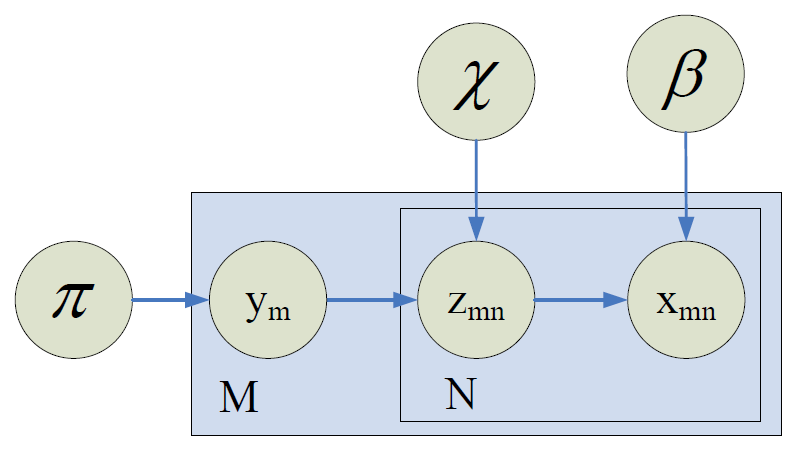
\includegraphics[scale=0.4]{lda.png}
\end{center}
\caption{The MGMM LDA model)}\label{ldamodel}
\end{figure}


\begin{algorithm}
\caption{MGMM Generating Process}
\label{algoGenerate}
\begin{algorithmic}[1]
\For{$m = 1$ to $M$ }
\State Choose a group type $Y_m \in \{1, ..., T\}, Y_m \sim \mathcal{M}(\pi)$  
\State let the topic distribution is $\theta_m = \chi_{Y_m}$
\State Choose number of points $N_m$ for group $G_m$
\For{$n = 1$ to $N_m$}
\State \mbox{Choose a topic $Z_{m,n} \in \{1,...,K\}, Z_{m,n} \sim \mathcal{M}(\theta_m)$}
\State Generate feature $X_{m,n} \sim \mathcal{N}(\beta_{Z_{m,n}}^\mu, \beta_{Z_{m,n}}^\Sigma)$
\EndFor
\EndFor
\end{algorithmic}
\end{algorithm}

\section{The Hierarchical Model}\label{sec:model}

In this section we describe the Mixture of Gaussian Mixture Model (MGMM) \cite{xiong2011hierarchical} for detecting group anomalies. The graphical representation is shown in figure \ref{ldamodel}. We have one set of observed variables $X_{m,n}$ and two sets of hidden variables $Y_m$ and $Z_{m,n}$. We have three parameters: $\pi$  is the multinomial parameter representing the normal group type distributions, $\chi = \{\chi_1, \chi_2, ..., \chi_T\}$ is the set of $T$ multinomial parameters representing topic proportions for the $T$ normal group types and $\beta=\{\beta_k^\mu, \beta_k^\Sigma\}_{k=1}^K$ is the possible means and covariance matrices. The generative process for the MGMM model is given in algorithm \ref{algoGenerate}.


\section{Inference and Learning}\label{sec:inferandlearn}
Given the observed data $X_{m,n}$, we need to infer the parameters $\Theta = \{\pi,\chi,\beta\}$. Once we learn the parameters we can easily calculate the likelihood of each group i.e. users and hence can find the anomalous groups or users. Let, all the points in a group $G_m=\{X_{m,n}\}_{n=1}^{N_m}$ and $Z_m=\{Z_{m,n}\}_{n=1}^{N_m}$. The joint likelihood of the latent and observed variables of a group $G_m$ can be written as:
\begin{align}
&P(Y_m, Z_m, G_m|\pi,\chi,\beta)\notag\\
&=P(Y_m|\pi)\prod\limits_{n=1}^{N_m}P(Z_{m,n}|Y_m,\chi)P(X_{m,n}|Z_{m,n},\beta)\\
&=\pi_{Y_m}\prod\limits_{n=1}^{N_m}\chi_{(Y_m,Z_{m,n})}\mathcal{N}(X_{m,n}|\beta_{Z_{m,n}}^\mu, \beta_{Z_{m,n}}^\Sigma)
\end{align}

Now, the marginal likelihood of the observations in group $G_m=\{X_{m,n}\}_{n=1}^{N_m}$ is:
\begin{align}
&P(G_m|\pi,\chi,\beta)\notag\\
&=\sum\limits_{t=1}^T\pi_t\prod\limits_{n=1}^{N_m}\sum\limits_{k=1}^K\chi_{(Y_m,Z_{m,n})}\mathcal{N}(X_{m,n}|\beta_{Z_{m,n}}^\mu, \beta_{Z_{m,n}}^\Sigma)
\end{align}
To learn the parameters using maximum likelihood estimation, we want:
\begin{align}
\arg\max\limits_{\pi,\chi,\beta}\prod\limits_{m=1}^MP(G_m|\pi,\chi,\beta)
\end{align}

Since, the traditional EM is intractable here, the variational approach is used. We need only to maximize the lower bound of the function.
Denote the hyper parameters by $\Theta = \{\pi, \chi,\beta\}$ .Using Jensen inqeality it is given by. 
\begin{align}
&\sum_{m=1}^{M}log P(G_m | \Theta)
\geq \sum\limits_{m=1}^{M} \int d(Y,Z)q_m(Y,Z) log\frac{P(Y,Z,G_m |\Theta)}{q_{m}(Y,Z)}
\end{align}
\begin{align}
=\sum\limits_{m=1}^{M} E[log P(Y,Z,G_m|\Theta)] - E_{q_m} [log q_m (Y,Z)]
\end{align}
So, this posterior distribution has intractable form, this instead we will solve the approximate maximization of the surrogate function for the free parameters.
\begin{align}
 \arg\max\limits_{\Theta,\{q_m\}}=\sum\limits_{m=1}^{M} E[log P(Y,Z,G_m|\Theta)] - E_{q_m} [log q_m (Y,Z)]
\end{align}
The surrogate distribution in special parameter is given by,
\begin{align}
 q(Y_m,Z_m | \gamma_m,\phi_m) = q(Y_m|\gamma_m) \prod_{n=1}^{N_m} q(Z_{m,n}|\phi_{m,n})
\end{align}
Here the $\gamma_m$ and $\phi_m$ are the variational parameters.
Then we have a variational learning problem to solve with following form
\begin{align}
\arg\max\limits_{\{\gamma_m\},\{ \phi_m \},\Theta}\sum_{m=1}^{M} L_m (\gamma_m,\phi_m,\Theta)
\end{align}
where 
\begin{align}
L_m (\gamma_m,\phi_m,\Theta ; \pi,\chi,\beta) = \sum\limits_{m=1}^{M}
E_q[log P(Y_m,Z_m,G_m|\pi,\chi,\beta)] - E_{q} [log q (Y_m,Z_m)] 
\end{align}
Then maximizing the $L_m$ function gives the estimation of the parameters. For detail \cite{xiong2011hierarchical}
\begin{align}
\phi_{m,n,k}^{*} = \frac{exp(\sum\limits_{t=1}^T\gamma_{m,t}log\chi_{t,k} + log P(X_{m,n}|\beta_k)}{\sum\limits_{j=1}^T exp(log\gamma_{m,t}log\chi_{t,j} + log P(X_{m,n}|\beta_j))}
\end{align}
\begin{align}
\gamma_{m,t}^* = \frac{exp(log\pi_t + \sum\limits_{n=1}^N\sum\limits_{k=1}^K \phi_{m,n,k}+log\chi_{t,k})}{\sum\limits_{\tau=1}^T exp(log \pi _\tau + \sum\limits_{n=1}^N\sum\limits_{\tau=1}^T \phi_{m,n,k}+log\chi_{\tau,k})}
\end{align}

\begin{align}
\pi_t^* = (\sum\limits_{\tau=1}^T\sum\limits_{m=1}^M \gamma_{m,\tau})^{-1}\sum\limits_{m=1}^M \gamma_{m,t}
\end{align}
\begin{align}
\chi_{t,k}^* = (\sum\limits_{j=1}^K\sum\limits_{m=1}^M \gamma_{m,t} \sum\limits_{n=1}^{N_m}\phi_{m,n,j} )^{-1} \sum\limits_{m=1}^M \gamma_{m,t} \sum\limits_{n=1}^{N_m}\phi_{m,n,k}
\end{align}
Finally to calculate $\beta$ we need to solve
\begin{align}
\arg\max\limits_{\beta_k}\sum\limits_{m=1}^M \sum\limits_{n=1}^{N_m}\sum\limits_{k=}^K\phi_{m,n,k} log P(X_{m,n}|\beta_k)
\end{align}


\begin{figure}
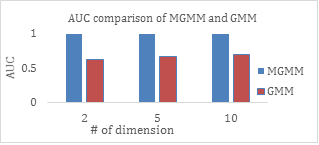
\includegraphics{synthetic.png}
\caption{AUC of group anomaly detector( MGMM) with point anomaly detector (GMM)}
\label{syntheticresult}
\end{figure}

\section{Experiments}\label{sec:experiments}
\subsection{Synthetic dataset}
Gaussian Mixture Model (GMM) using synthetic dataset. We generated synthetic dataset using the generative algorithm described in algorithm \ref{algoGenerate}. For the experiments we generated synthetic datasets of 50 groups and 5000 points with 2, 5 and 10 dimensions. Then we inject two types of anomalous groups. The first types are point wise anomaly group with distribution of $ \mathcal{N} (0,1) $ and the second types are group anomalies with same mean and covariance matrix as the normal groups but with different topic proportions. Then we assign each group different group membership id to identify their groups.
To compare the performance of the point wise anomaly detector GMM with the group anomaly detector MGMM, fist we compute individual likelihood using the GMM, then we aggregated the score of individual points in the same groups. We took log sum of the individual scores to get the group wise likelihood for the GMM.  Then, we compare the result with the score of group likelihood generated from the MGMM of the 50 groups. The overall performance comparison is shown in figure \ref{syntheticresult}.


The results in figure \ref{syntheticresult} shows that the group anomaly detection achieved better result across all the datasets in all dimensions compared to the point wise Gaussian mixture Model.

\begin{figure*}
\begin{center}
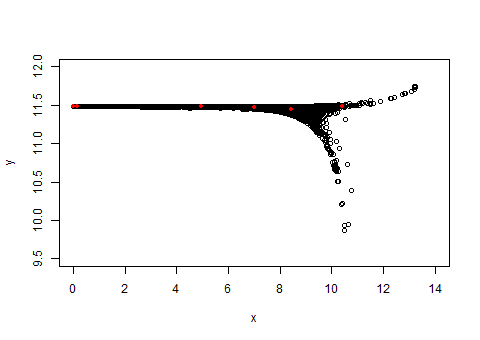
\includegraphics[bb = 0 15 460 290,clip=true,scale=0.9]{Topics.png}
\end{center}
\caption{Scatter plot of all the points from all the groups along with the 6 topic centers learned (Red points)}\label{learnedTopics}
\end{figure*}

\subsection{ADAMS Intrusion Detection Dataset}
This dataset contains information of 5691 users of a corporate network. All activities of these users are monitored and en-coded into 69 features. The activities were recorded by date i.e. for each day we have one feature vector corresponding to one user, which we can call a user day. We run the group anomaly detection on a collection of such user days for the month of April 2013. The complete dataset contains around 170K user day instances. Our goal is to identify the anomalous users i.e. the users those are actually threat. The ground truth anomalies were inserted by the Red Team Inserts, a team whose job is to insert anomalies in a realistic way to make them appear as they occurred naturally. To run the group anomaly detector we treated each user is a group where each group i.e. user contains 30 user days. Our goal is to detect users whose user day distribution appears anomalous i.e. to detect the groups those distributions are different than normal groups distributions. The point here is that the individual user days might not be anomalous but when considered as a group they might appear normal.

We assume that each user group is coming from T normal group types where under each group the user days belongs to one of the K global topic those are shared among the entire dataset.

\begin{figure*}
\begin{center}
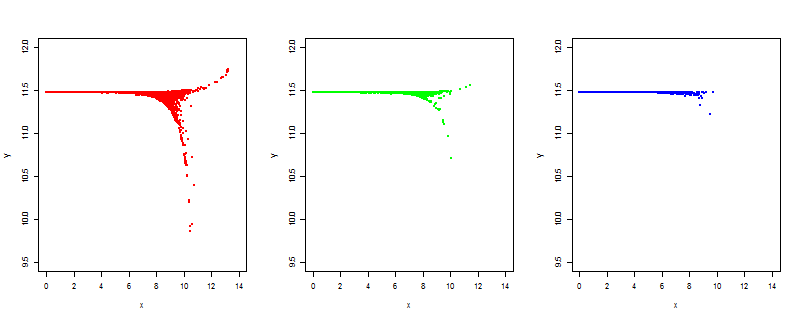
\includegraphics[bb = 0 5 785 285,clip=true,scale=0.65]{Groups.png}
\end{center}
\caption{Scatter plot of the points assigned to group type 1 (left), group type 2 (center) and group type 3 (right). The hidden variables grouped types were inferred from the learned model parameters}\label{learnedGroups}
\end{figure*}

\subsubsection{Data Preprocessing:}
It is common to apply some dimensionality reduction techniques to the data before applying the anomaly detection, since the dataset might contain some low variance and redundant dimensions. We used PCA to reduce our data. First, we applied PCA and retained only the principle components those represent 95\% of the variance and it reduced the dataset from 69 dimension to just 2 dimensions. We also tried retaining 99\% variance, which reduced the data dimension to 4. And also before applying PCA we scaled the data to have unit variance and then applied the PCA, which reduced the dimension 69 to 38. We run the group anomaly detection on these three reduced datasets and observed that they produce almost similar performance in terms of AUC. Hence, we only report and discus the results found from the reduced 2D data, since it will allow us to get more insight into the datasets.


\subsubsection{Topics and Groups learned:} We choose different values of T and K and computed the corresponding AUC. We got the best AUC of 0.78 when used T = 3 and K = 6, i.e. 3 normal group types and 6 topics. First we show the scattered plot of the reduced 2D dataset in Figure \ref{learnedTopics} along with the 6 topic centers (red dots) found after learning the parameters. It is worth to mention that we translated the points to make all the coordinates positive and then applied log on both x and y axis, hence the x and y axis in Figure \ref{learnedTopics} are in logarithmic scale.

We inferred the group types for each of the users from the learned parameters. We show the data points assigned in three normal group types in figure \ref{learnedGroups}. We observe that most of the groups are assigned to group type 1 and less number of groups are assigned to group type 3.

In figure \ref{distTopic} above we show the distribution of topics under each group types. We see that most of the points are generated from topic 1 and topic 6 and only a few points are generated from topic 2. Group type 3 is sparse i.e. contains most of the points from topic 1 and 6 and almost none from other four topics.

\begin{figure*}
\begin{center}
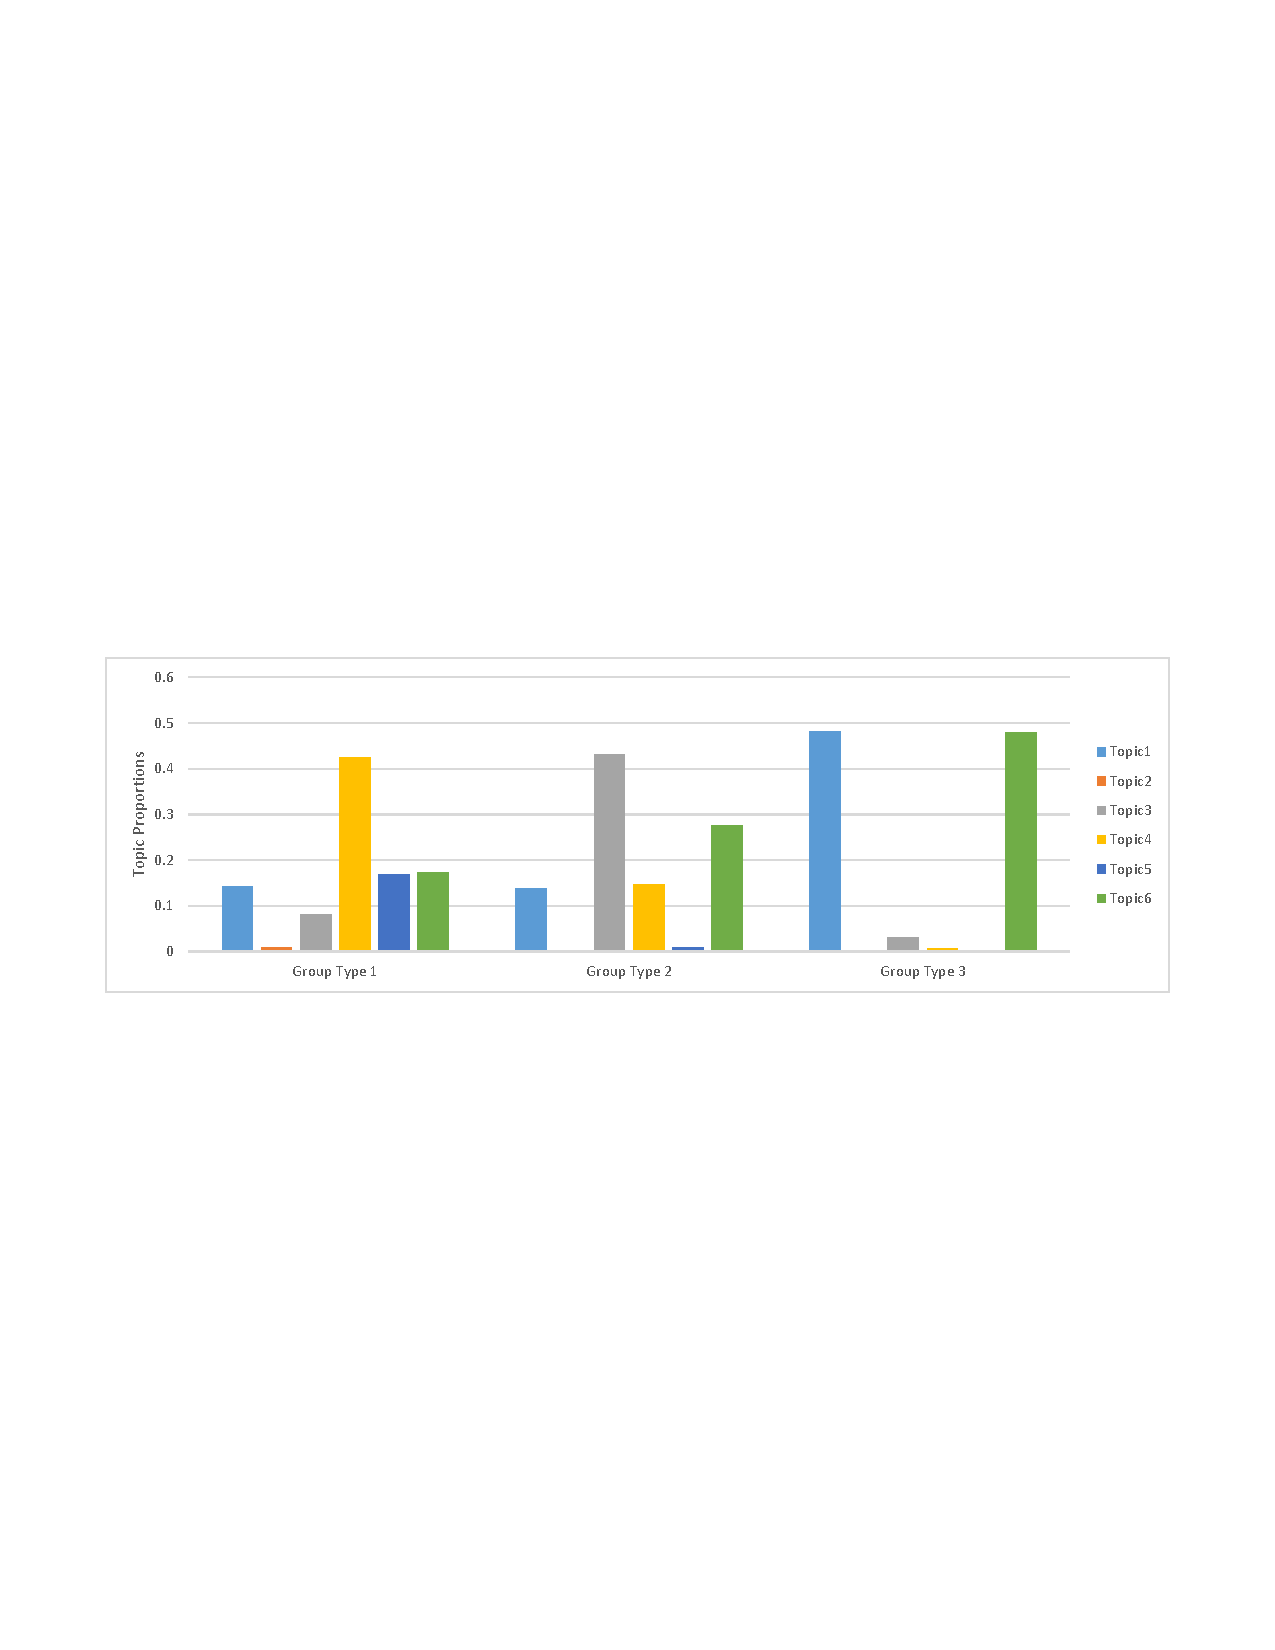
\includegraphics[bb = 55 320 560 470,clip=true,width=1\textwidth]{T3_K6_Chi.pdf}
\end{center}
\caption{Distribution of topics under different group types}\label{distTopic}
\end{figure*}


\subsubsection{Effect of number of normal groups:} We want to see how the performance of the anomaly detector varies when we choose different number of normal group types. In figure \ref{effectGroups} we plot the number of normal groups in x axis and in y axis we put average AUC of different topics.

We observe that in figure \ref{effectGroups}, when we increase number of groups there is a decrease in performance, i.e. AUC decreases and best performance is achieved when using number of normal group types equals 2. The performance degrades when we increase number of normal group types is because anomalous groups will tend to fall under one of these groups which will give more false negatives.

\begin{figure}
\begin{center}
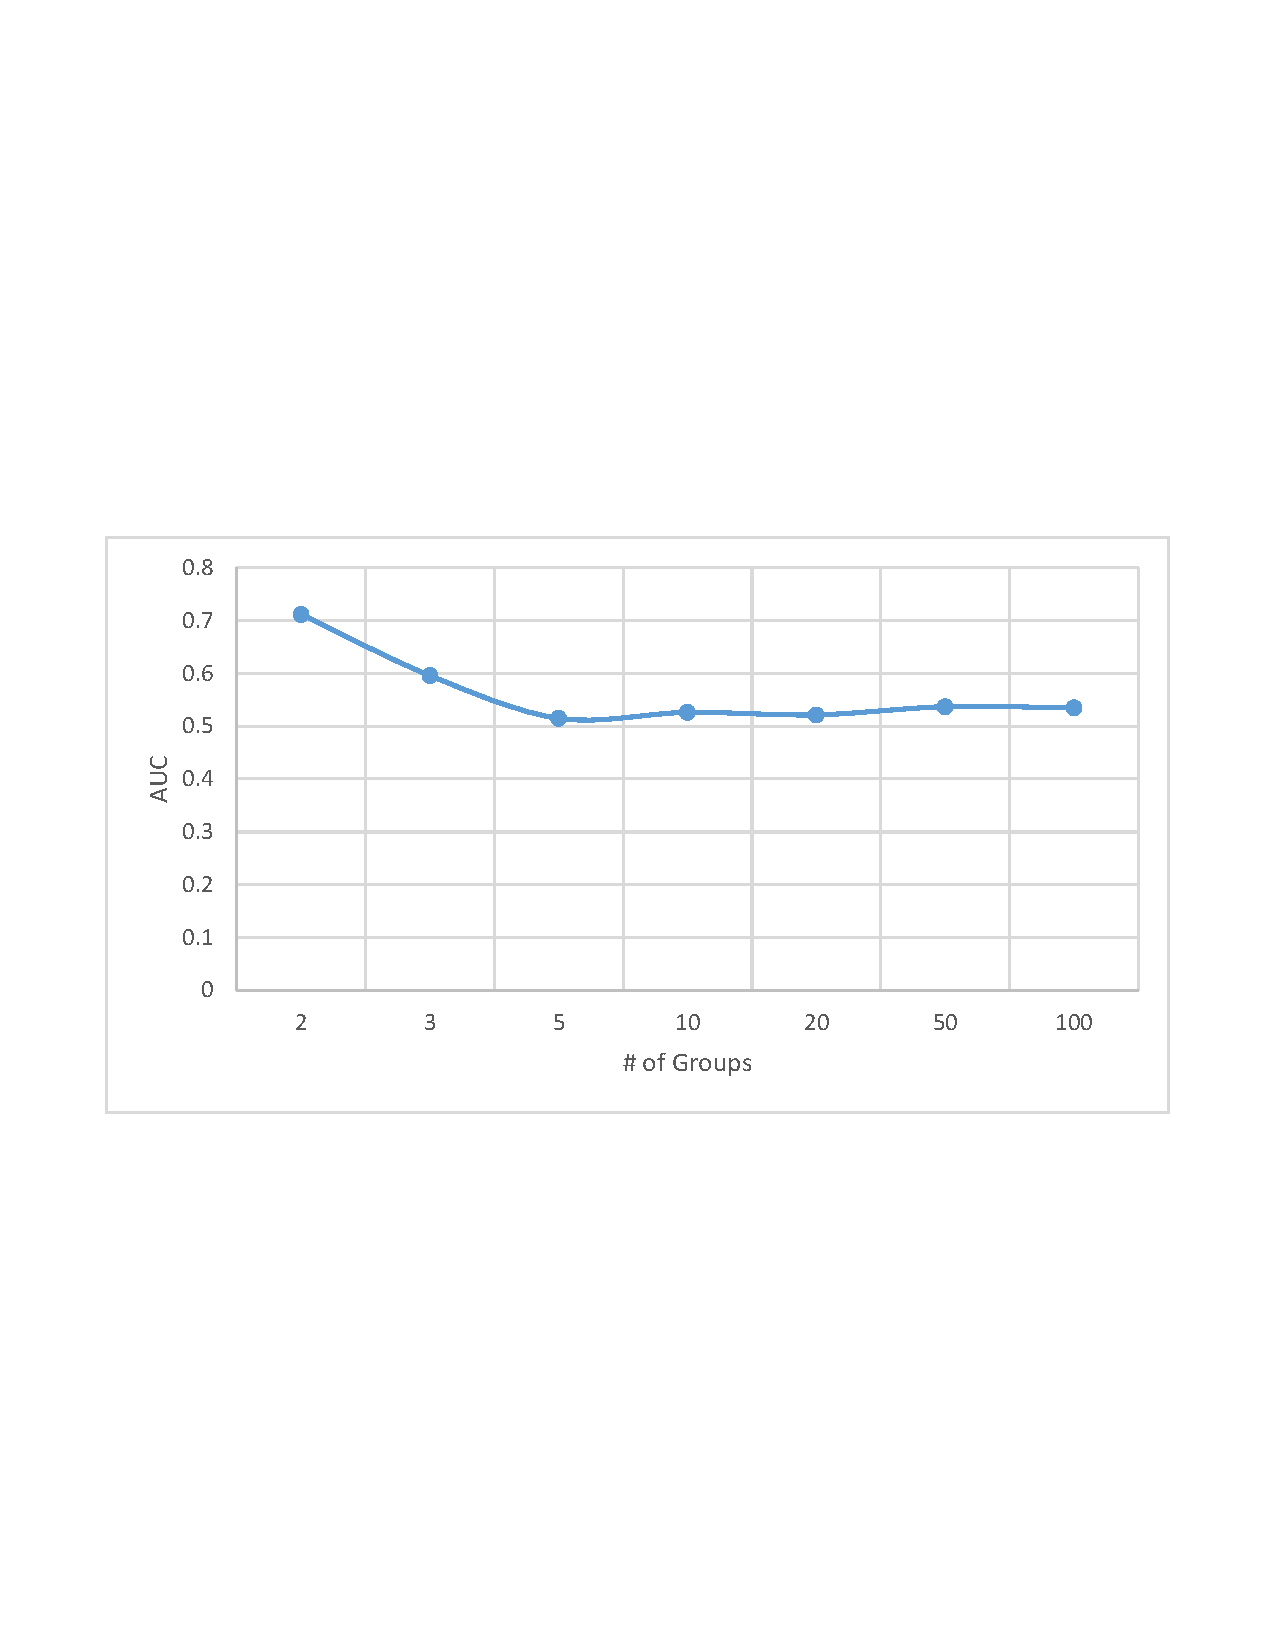
\includegraphics[bb = 70 270 550 530,clip=true,width=0.45\textwidth]{ResultGroupVsAUC.pdf}
\end{center}
\caption{Effect of number of groups in performance of anomaly detector}\label{effectGroups}
\end{figure}

\begin{figure}
\begin{center}
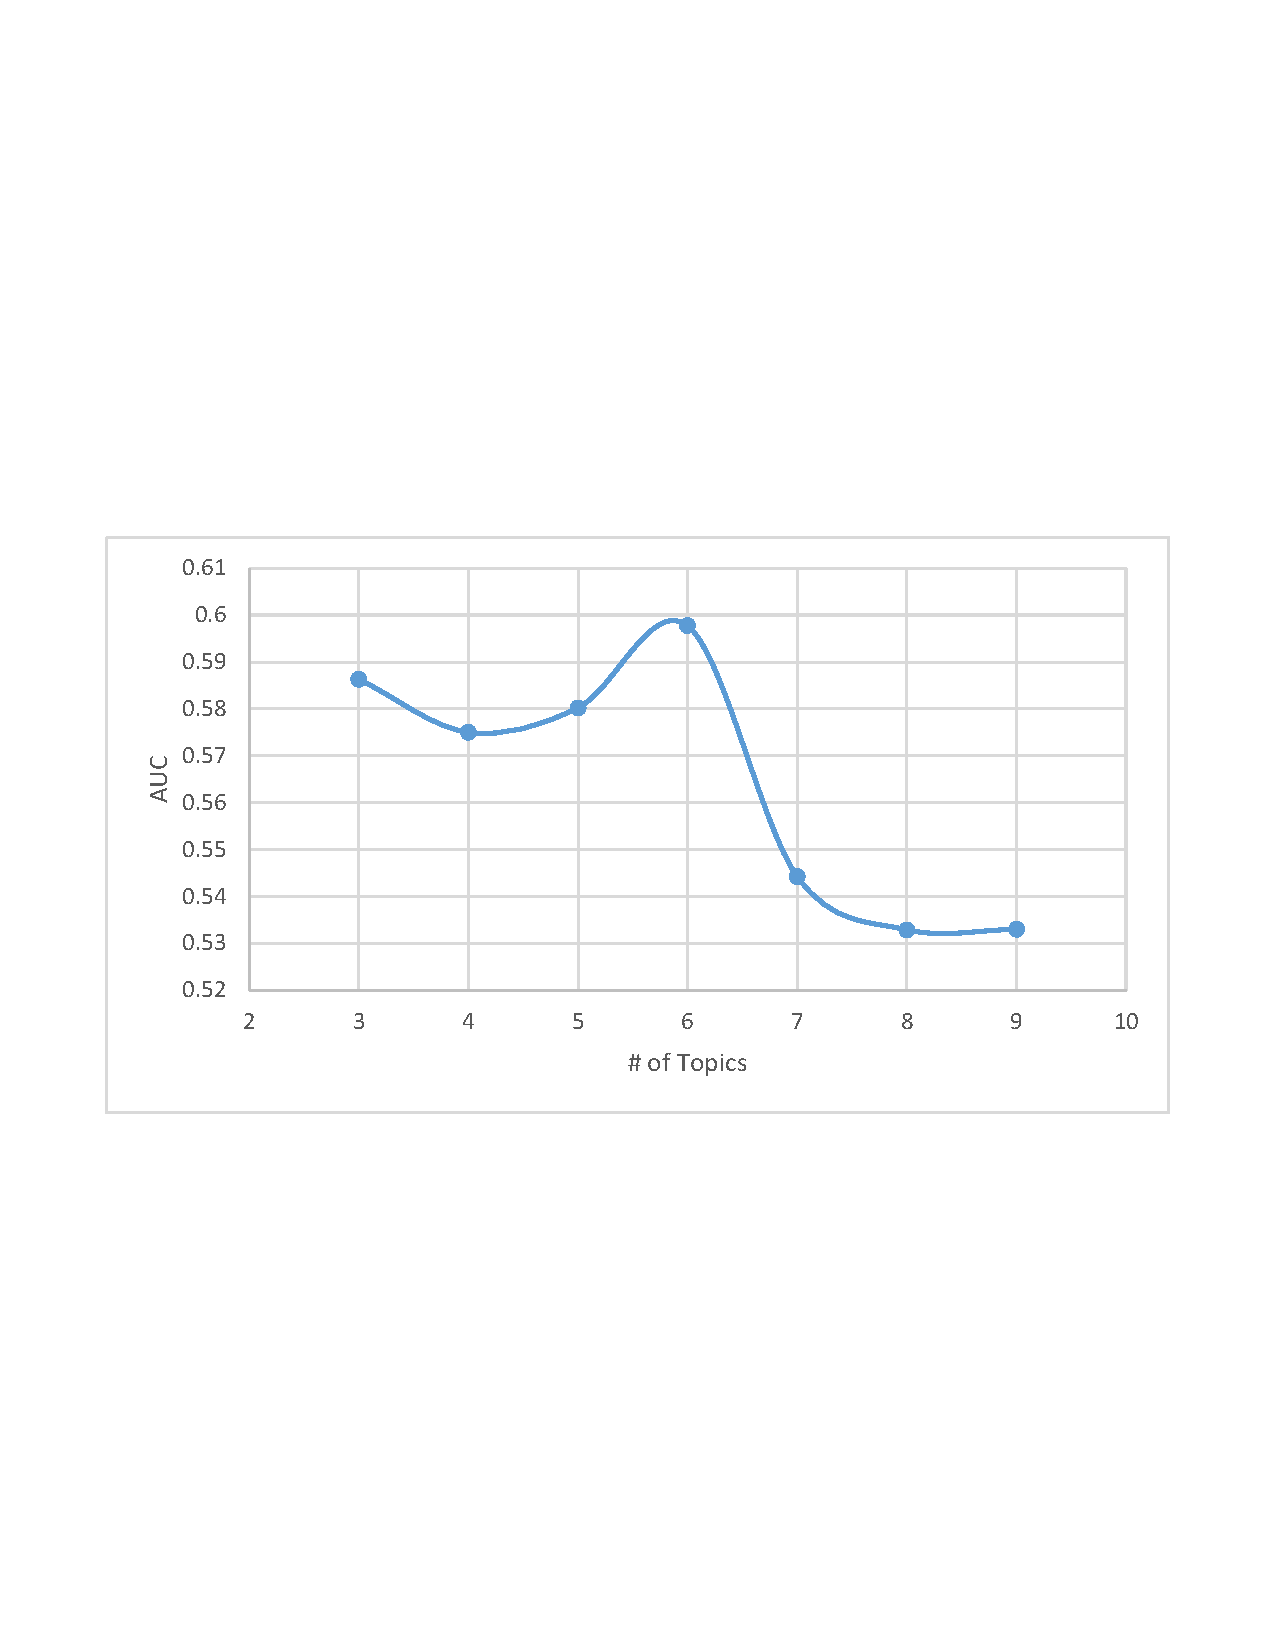
\includegraphics[bb = 70 270 550 530,clip=true,width=0.45\textwidth]{ResultTopicVsAuc.pdf}
\end{center}
\caption{Effect of number of topics in performance of anomaly detector}\label{effectTopics}
\end{figure}


\subsubsection{Effect of number of topics:} In figure \ref{effectTopics} below we plot number of topics vs. average AUC in different group numbers. Choosing small number of topics does not help identifying anomalous groups. Also large number of topics does not. We observed that the best performance is achieved when number of topics is 6. The reason is that when we have very small number of topics the group types will tend to produce similar topic distributions hence will get lots of false negatives, on the other hand if we have large number of topics the distributions will be mostly anomalous and will produce large number of false positives. In both of the cases the anomaly detector will perform badly.

\subsection{Weather temperature dataset}
In this experiment, we tested the performance of the group anomaly detection in air temperature weather data from Oklahoma state weather stations. The weather station have readingss on every 5 minutes intervals, which constitute 288 readings in each day. In our case we are interested in the whole day readings of 288 dimensions.

In order to prepare dataset for group anomaly detection problem, first we selected 12 weather stations which are not far apart. We chose a sample weather station i.e. 'SPEN', then we collect data from all weather stations which are under 40 miles radius from it. Our assumption is, stations which are close to each other will have highly correlated readings in a specific time interval. For example, in a particular day and time, each station will have similar readings. Using this assumption, we proposed a grouping method based on days, where each group contains readings from all stations in the particular day. So, we formulate total 365 groups, each containing readings from 12 weather stations.

In this domain anomalous event occurs when there is failure in a particular weather station. So, a group can be anomaly if it has one or more faulty readings from its station in that day. Here our objective is to detect these anomalies groups (days) by exploiting the grouping structure of the readings. To perform that first we reduced the dimension of the data using PCA from 288 to 4 dimension by retaining 95\% variance of the features. The problem with the original dimension was that the model parameters can not be inferred for the high dimensional space due to the constrain that one of the Gaussian parameter i.e. the covariance matrix need to be positive definite.

We tested our proposed hierarchal model on the dataset to find the likelihood score of each groups using different topics and group types learned. Our assumption is if there is a faulty readings from one of the station in a particular day, this will make the group likelihood low compare to others.

For the experiments we used different parameter set of Topic and group type, $T=2, 3, 5, 10, 20 and 100$ and $K= 3 to 7$.  The performance is measured using area under the ROC curve (AUC) of finding the anomalies in the data set. For the ground truth of the dataset we used the label for each day readings of a particular station. To generate ground truth for the groups, we assumed if there is one or more faulty stations in that day the group is flagged as faulty.

\begin{figure}
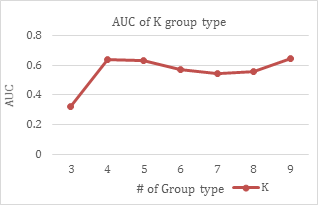
\includegraphics{grouptype.png}
\caption{AUC across different number of group type}
\label{weathergroupauc}
\end{figure}

\begin{figure}
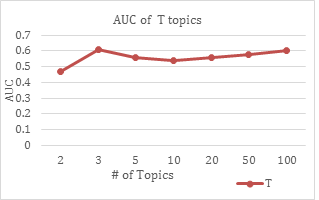
\includegraphics{topic.png}
\caption{AUC across different number of topics}
\label{weathertopicauc}
\end{figure}

The overall result in figure \ref{weathergroupauc} and \ref{weathertopicauc} show, the anomaly detection performance of the model is not really good. There reason could be because in the dataset the number of group members are small. For example, in this dataset in each group we have 12 points from the 12 weather station. The performance might be increased if we increase number of stations. But, increasing number of station with further distance might decrease the correlation as well, which leads to an non-informative grouping. But, in comparison the algorithm achieves better performance for number of Topic $K=5$ and number of normal group types $T=4$. On the other hand, the result in the weather data shows, after certain topic configuration, the accuracy tends to decrease as we increase number of topics or group type.


Then from the AUC result we took the best result from number of group type $T=4$ and number of topics $K=5$ which is around 0.72. Using this configuration we compute the topic proportion of each group type, which is shown in the figure \ref{weathertopicprop}.

\begin{figure}
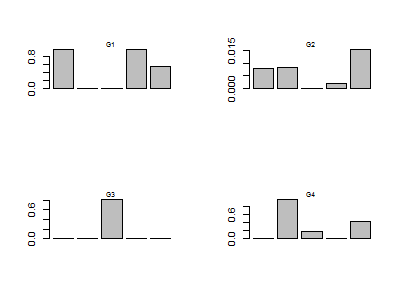
\includegraphics[scale=0.6]{topicprop.png}
\caption{Topic proportion of different group types}
\label{weathertopicprop}
\end{figure}

The figure \ref{weathertopicprop} show how each group type are different in their topic composition. For example, Group type 1 are mostly from topic 1, 4 and 5, and Group type 3 are mostly composed of topic 3.

\section{Conclusion}\label{sec:conclusion}
We observed from the experimental results that our hypothesis that Group anomaly detection can perform well on detecting group anomaly from real domains actually failed. We only observed good performance on the synthetic datasets. The main reason for bad performance in real domain we think are as follows:
\begin{itemize}
\item The model in figure \ref{ldamodel} is very simple to deal with complex domains, we see that it only involves some multinomial and Gaussian distributions in data generation process.
\item We observe that the number of points in each group in both ADAMS and weather datasets are very small i.e. 30 and 12. These might prevented to learn a stable topic distribution under each group
\item Instead of learning topics per group, the topics are learned globally, which might prevented to learn a flexible enough model
\item The fixed set of topic proportions might limited the model to learn complex topic proportions per group
\end{itemize}
As a future work, it would be interesting to see how the improved model i.e. the Flexible Genre Model (FGM) proposed in \cite{xiong2011group} performs on the ADAMS and weather dataset.

\bibliographystyle{aaai}\bibliography{bibgroupanomaly}

\end{document}
